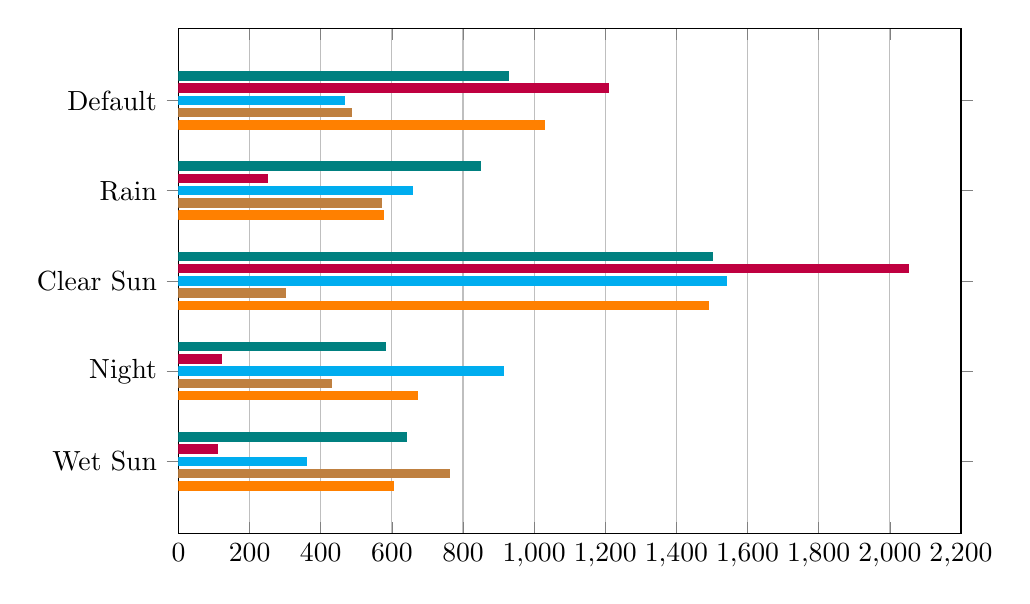
\begin{tikzpicture}
  \begin{axis}
      [
        width  = .95\textwidth,
        height = 8cm,
        xbar = .05cm,
        bar width=3pt,
        xmajorgrids = true,
        xmin = 0, 
        xmax = 2200,
        ytick=data,
        %enlarge x limits = {value = .25, upper},
        enlarge y limits = {abs = .8},
        yticklabels={Wet Sun, Night, Clear Sun, Rain, Default}
      ]
      %Run 1 bei allen
      \addplot[xbar][style={orange,fill=orange,mark=none}]
      coordinates {(604,0) (672,1) (1491,2) (575,3) (1029,4)};
      %Run 2 bei allen
      \addplot[xbar][style={brown,fill=brown,mark=none}]
      coordinates {(763,0) (429,1) (301,2) (571,3) (486,4)};
      %Run 3 bei allen
      \addplot[xbar][style={cyan,fill=cyan,mark=none}]
      coordinates {(359,0) (915,1) (1540,2) (658,3) (466,4)};
      %Run 4 bei allen
      \addplot[xbar][style={purple,fill=purple,mark=none}]
      coordinates {(109,0) (121,1) (2052,2) (249,3) (1208,4)};
      %Run 5 bei allen
      \addplot[xbar][style={teal,fill=teal,mark=none}]
      coordinates {(641,0) (582,1) (1500,2) (850,3) (929,4)};
  \end{axis}
\end{tikzpicture}